\section{Implementation and Experiments}

\subsection{Clause Reduction with $\IUIP$}
To evaluate $\IUIP$'s effectiveness as a clause reduction technique, we implement  $\IUIPPURE$ and $\IUIPMIN$ with Control-I-UIP and Early Stopping rules in Sec~\ref{sec:i-uip} on top of \text{\MapleBase} \cite{}, the winner of SAT Race 2015 application track.  We than compare the performance of the baseline $\MapleBase$ with $\MapleIUIPPURE$ and $\MapleIUIMIN$ on the full set of benchmarks from SAT RACE 2019 main track.

The benchmark contains 400 instances divided into two groups of 200, new and old, representing historical instances and fresh instances in the 2019 race, respectively. I partition the old group instances into six partitions of size 30 and one partition of size 20. Each partition is then assigned to a XeonE5-2 CPU node with 16 cores (2 sockets 8 cores  and  1 thread) and 96649 MB memory. The new group is partitioned based on their contributor (e.g. Heule contributed 22 matrix multiplication instances), and each partition is assigned to a aforementioned CPU node. To speed up the experiment, we allow a CPU node to solver at most seven instances concurrently. 

Beside solved instances count and PAR-2 score, we additionally measure the average clause length and clause reduction ratio (both cumulative and non-cumulative)\footnote{The cumulative reduction ratio is obtained through learning all clauses with the target learning scheme; Therefore, the reduction is cumulative. The non-cumulative reduction ratio is obtained by running the target scheme for measurement only (the minimized 1-UIP clause is learned); Therefore, the reduction is not cumulative. }  for each instances. For $\MapleIUIPPURE$  and $\MapleIUIMIN$, we also captures the $\IUIP$ learning attempted rate and success rate.

\begin{figure} 
\begin{center}
\begin{tabular}{ | m{3.3cm} | m{2cm}| m{2cm} | m{2cm} | m{2.7cm} | } 
\hline
Solver & \# solved & PAR-2 & Clause Size & Cl Reduction\% \\ 
\hline
$\MapleBase$ & 221 (132, 89) & 5018.89 & 62.6 & 36.53\% \\ 
\hline
$\MapleIUIPPURE$ & \textbf{228} (135, 93) & \nf{4867.37} & 49.88 & 41.6\%  (42.72\%)\\ 
\hline
$\MapleIUIMIN$ & 226 (135, 91) & 4890.67 & \textbf{45.2} & \textbf{47.8\% (51.19\%)}\\ 
\hline
\end{tabular}
\end{center}
\caption{Benchmark results of $\MapleBase$ , $\MapleIUIPPURE$  and $\MapleIUIMIN$ on SAT2019 race main track.
CL Reduction\% is the clause size reduction ratio comparing to non-minimized 1-UIP clauses, and the values in the brackets are the non-cumulative reduction ratio.}
\label{fig:t1}
\end{figure}

Fig.~\ref{fig:t1} shows that $\IUIPPURE$ ($\IUIPPURE$) solved seven (five) more instances than the baseline solver with lower PAR-2 scores. $\IUIPPURE$ has marginally lower PAR-2 score than $\IUIPPURE$. Both $\IUIPPURE$ and $\IUIPMIN$ produce clause with significantly smaller size than 1-UIP by  20.4\% and 27.7\%, respectively. Fig.~\ref{fig:len_pdf} shows the probability density distribution (PDF) of the relative clause size of both i-uip learning schemes ($\IUIPPURE$ in red and $\IUIPMIN$ in green) for each instance. $\IUIPPURE$ ($\IUIPMIN$) produces shorter clauses for 77.7\% (88.5\%) of instances, and average relative reduction from 1-UIP is 16.7\% (18.6\%). Fig.~\ref{fig:len_compare} compares the absolute clause size of $\IUIPMIN$, $\IUIPPURE$ and 1-UIP, and it shows that both i-UIP learning schemes in general produce the smaller clauses, and the size reduction is more significant for instances with large average 1-UIP clause size. Moreover, $\IUIPMIN$ clauses (indicated in green) is consistently smaller than $\IUIPPURE$ clauses.

\begin{figure}
    \centering
    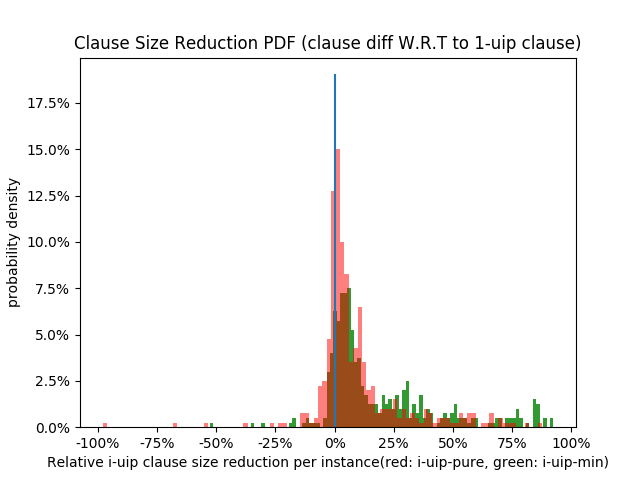
\includegraphics[width=0.8\textwidth,natwidth=610,natheight=642]{figures/clause_reduction_PDF.png}
     \caption{ Relative clause size reduction distribution. X axis indicates the relative size of difference between i-uip and 1-uip clauses (calculated as $\dfrac{|\oneUIPClause|-|\iUIPClause|}{|\oneUIPClause|}$ ) for each instance, and Y axis shows the probability density.}
     \label{fig:len_pdf}
\end{figure}
\begin{figure} \label{fig:len_compare}
    \centering
    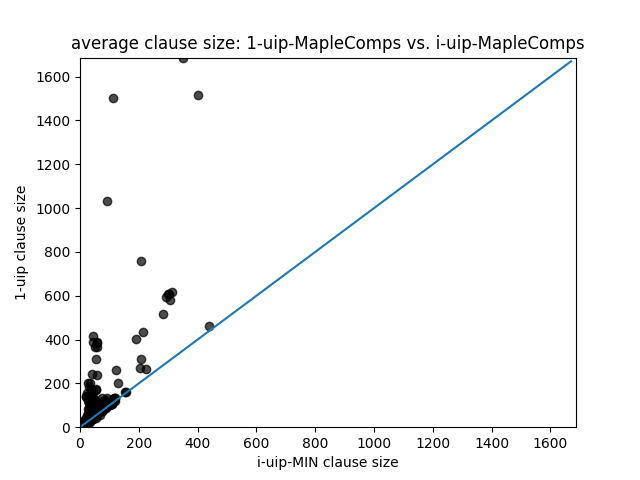
\includegraphics[width=0.8\textwidth,natwidth=610,natheight=642]{i-uip-sizes-compare.png}
    \caption{Average clause size comparison plot. Each point in the plot represents an instance. X and Y axis shows the clause length from $\IUIP$ and 1-UIP, respectively. Each green (red) dot represents an compared instance between $\MapleBase$ and $\MapleIUIMIN$ ($\IUIPPURE$). }
    \label{fig:len_compare}
\end{figure}
\nf{ Do we need this?
We additionally looked at the 14 instances solved by $\IUIPMIN$ but not by 1-UIP. $\IUIPMIN$ produces smaller clauses for all of them with average relative reduction of 22\% and maximum 77\% (30 vs 135). Seven out of 14 instances has size relative reduction over 30\%. For the 9 instances solved by 1-UIP but not by $\IUIPMIN$, $\IUIPMIN$ only produce smaller clause for three instances and with average relative reduction of 3.3\%.}


$\IUIPMIN$ outperformed $\IUIPPURE$ in clause size.  This results agrees with our observation in Fig.~\ref{fig:t2}: $\IUIPMIN$ attempted $\IUIP$ learning more frequently, and it is more likely to succeed. Remark that the success of $\IUIP$ learning is determined by the size of the learned i-UIP clause $\iUIPClause$, and the $\IUIP$ learning frequency is also indirectly controlled by $\IUIP$'s success rate from the previous restart interval. The results indicates  $\IUIPMIN$ shortened $\iUIPClause$'s size through further resolutions of $\iUIPClause$ at non-unique implication decision level. 

\begin{figure} 
\begin{center} 
\begin{tabular}{ | m{3.5cm} | m{5cm}| m{3.5cm} | } 
\hline
Solver & $\IUIP$ attempt rate & $\IUIP$ success rate  \\ 
\hline
$\MapleIUIPPURE$ & 16.1\% & 43.4\% \\ 
\hline
$\MapleIUIMIN$ & 28.8\% & 59.3\% \\ 
\hline
\end{tabular}
\end{center}
\caption{Compare $\IUIPPURE$ and $\IUIPMIN$ i-uip attempt rate and success rate. $\IUIPMIN$ scheme attempted $\IUIP$ more frequently, and it is more likely to successfully produce smaller $\iUIPClause$ clause .}
\label{fig:t2}
\end{figure}

A solver produce smaller clauses can construct smaller proofs. For UNSAT instances, we measure their DRUP\cite{} proof checking time as well as the size of the optimized DRUP proof. We used DART-trim \cite{} with 5000 timeout to check and optimize DRUP proofs. 

Fig.~\ref{fig:t3} shows that the optimized proof construct by $\IUIPMIN$ and $\IUIPPURE$ are significantly smaller than 1-UIP proofs. The relative proof size reduction roughly correlates to the average clause size reduction. Fig.~\ref{fig:proof_compare} shows the absolute proof size comparison results. 

\begin{figure} 
\begin{center} 
\begin{tabular}{ | m{3.5cm} | m{5cm}| m{3.5cm} | } 
\hline
Solver & optimized proof size (MB) & relative reduction size  \\ 
\hline
$\MapleBase$ & 613.9 & 0  \\ 
\hline
$\MapleIUIPPURE$ & 487.2 & 6.90\% \\ 
\hline
$\MapleIUIMIN$ & 413.2 & 17.18\% \\ 
\hline
\end{tabular}
\end{center}
\caption{Optimized UNSAT proof comparison for 1-UIP $\IUIPPURE$ and $\IUIPMIN$. Optimized proof size measures the average absolute proof size in MB, and relative reduction size measures the average relative reduction for all UNSAT instances.}
\label{fig:t3}
\end{figure}

\begin{figure}
    \centering
    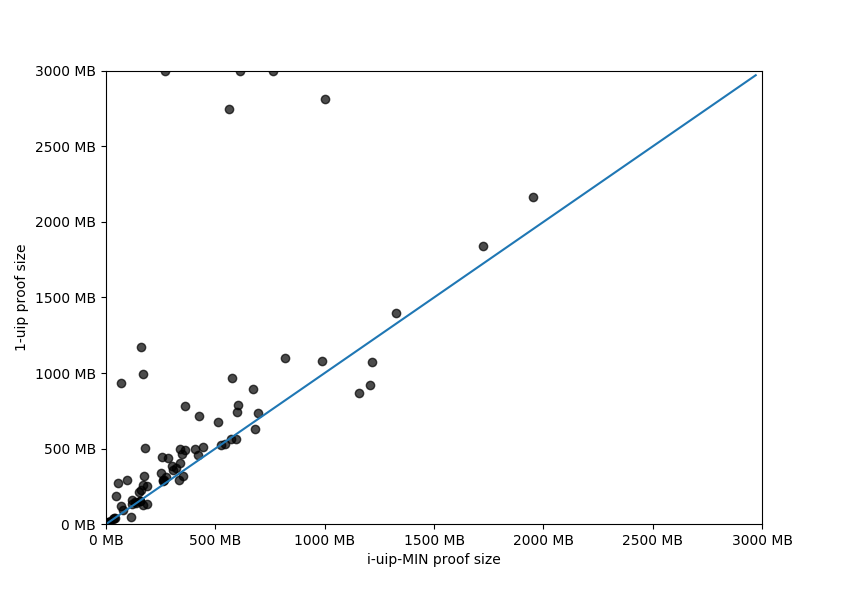
\includegraphics[width=0.8\textwidth,natwidth=610,natheight=642]{proof_size_compare.png}
    \caption{Average optimized proof size between 1-uip and $\IUIPMIN$.}
    \label{fig:proof_compare}
\end{figure}


\begin{figure} 
\begin{center}
\begin{tabular}{ | m{3.5cm} | m{4cm}| m{2cm} | m{2.75cm} |  } 
\hline
Solver & \# solved (SAT, UNSAT) & PAR-2 & Avg clause Size \\ 
\hline
1-UIP & 221 (132, 89)  & 5018.89 & 62.6  \\ 
\hline
\nf{$\IUIPPURE$} &\textbf{228} (135, \nf{93}) & 4867.37 & 49.88 \\
\hline
$\IUIPMIN$ & 226 (135, 91) & 4890.67 & 45.2 \\ 
\hline
$\IUIPGreedy$ & 226 (135, 91)  & \textbf{4866.94} & 47.7 \\
\hline
$\IUIPActive$ & 225 (\textbf{138}, 87) & 4958.49 & 52..12 \\
\hline
$\IUIPDist$ & 223 (134, 89) & 5015.23 & \textbf{43.2} \\
\hline
\end{tabular}
\end{center}
\caption{Benchmark results of $\MapleBase$ with 1-UIP, $\IUIPPURE$, $\IUIPMIN$, $\IUIPGreedy$,
$\IUIPActive$, and $\IUIPDist$ on SAT2019 race main track.}
\label{fig:t4}
\end{figure}

\subsection{$\IUIP$ as a Practical Learning Scheme}
To evaluate $\IUIP$'s effectiveness as a clause learning scheme, we re-implement $\IUIPMIN$ on $\MapleBase$ with the extensions mentioned in section~\ref{sec:i-uip}. We evaluated 1-UIP learning and five $\IUIP$ configurations ( $\IUIPMIN$, $\IUIPPURE$, $\IUIPGreedy$, $\IUIPActive$, and $\IUIPDist$) on the SAT Race 2019 main track benchmark and reported solved instances, PAR-2 score and average clause size. 

Fig.~\ref{fig:t4} summarizes the result of the experiment. Learning scheme $\IUIPPURE$ solved the most overall instances (228) and the most UNSAT instances (93). $\IUIPGreedy$ had the lowest PAR-2 score. $\IUIPActive$ solved the most SAT instances (138). $\IUIPDist$ produced the shortest average clause size, but solved the second least instances, one more instance than the baseline 1-UIP learning. All configurations of $\IUIP$ outperformed the baseline 1-UIP scheme in solved instances, PAR-2 score and average clause size.


\subsection{$\IUIP$ on Modern SAT solvers}
To validate $\IUIP$ as a generalizable learning scheme on modern SAT solvers, we re-implement $\IUIP$ on the winners of 2017, 2018 and 2019 SAT Race\cite{} and $\expSAT$\cite{} ($\expSATShort$). $\expSATShort$ is a top ten solver from 2019 SAT race which uses random walk simulation to help branching. We chose $\expSATShort$ because 1) it is a top solver in the 2019 SAT Race without using chronological backtracking; 2) the combination of random walk simulation and variable activity branching heuristic allows our learning schemes to partially sidestep the problem of variable activity. For each solver, we compare the base 1-UIP learning scheme against $\IUIPPURE$, $\IUIPMIN$ and the top two $\IUIP$ variants, $\IUIPGreedy$ and $\IUIPActive$, on the SAT Race 2019 main track benchmark. We report solved instances, PAR-2 score and the average clause size.

\begin{figure} 
\begin{center}
\begin{tabular}{ | m{3.7cm} | m{4cm}| m{2cm} | m{2.75cm} |  } 
\hline
Solver & \# solved (SAT, UNSAT) & PAR-2 & Avg clause Size \\ 
\hline
SAT 2017 Winner & & & \\
$\MapleSeven$ & 232 (135, 97) & 4755.96 & 61.9  \\ 
\hline
$\MapleSeven$-i-pure & \textbf{244 (146, 98)} +12 & \textbf{4504.18} & 43.76 \\
\hline
$\MapleSeven$-i-min & 240 (144, 96) +8 & 4601.25 & \textbf{36.97} \\ 
\hline
$\MapleSeven$-i-greedy & 237 (140, 97) +5 & 4678.434 & 43.62 \\ 
\hline
$\MapleSeven$-i-inclusive & 234 (137, 97) +2 & 4718.03 & 37.96 \\
\hline
\hline
SAT 2018 Winner & & & \\
$\MapleEightShort$ & 236 (138, 98) & 4671.81 & 61.69 \\
\hline
$\MapleEightShort$-i-pure & \textbf{241} (\textbf{142, 99}) +5 & \textbf{4598.18} & 44.19 \\
\hline
$\MapleEightShort$-i-min & 236 (141, 95) +0 & 4683.92 & 38.05 \\ 
\hline
$\MapleEightShort$-i-greedy & 240 (141, \textbf{99}) +4 & 4626.99 & 41.16 \\
\hline
$\MapleEightShort$-i-inclusive & 240 (\textbf{142}, 98) +4 & 4602.13 & \textbf{37.52} \\
\hline
\hline
SAT 2019 Winner & & & \\
$\MapleNineShort$ & 238 (140, \textbf{98}) & 4531.24 & 60.91 \\
\hline
$\MapleNineShort$-i-pure & 238 (140, \textbf{98}) +0 & 4519.08 &  43.32\\
\hline
$\MapleNineShort$-i-min & 244 (\textbf{148}, 96) +6 & \textbf{4419.84} & \textbf{36.88} \\
\hline
$\MapleNineShort$-i-greedy & 243 (146, 97) + 5 & 4476.73 & 40.65 \\
\hline
$\MapleNineShort$-i-inclusive & \textbf{243} (\textbf{148}, 95) +5 & 4455.76 & 37.02 \\
\hline
\hline
SAT 2019 Competitor & & &\\
$\expSATShort$ & 237 (137, 100)  & 4628.96 & 63.19 \\
\hline
$\expSATShort$-i-pure & 235 (136, 99) -2  & 4668.96 & 48.26 \\
\hline
$\expSATShort$-i-min & 241 (143, 98) +4 & 4524.28 & 46.29 \\ 
\hline
$\expSATShort$-i-greedy & 244 (143, \textbf{101}) +7 & \textbf{4460.92} & 47.25 \\
\hline
$\expSATShort$-i-inclusive & \textbf{245} (\textbf{146}, 99) +8 & 4475.76 & \textbf{45.33} \\
\hline
\end{tabular}
\end{center}
\caption{Benchmark results of 1-UIP, $\IUIPPURE$. $\IUIPMIN$, $\IUIPGreedy$ and $\IUIPActive$ on SAT2019 race main track.}
\label{fig:t5}
\end{figure}

\nf{Benchmark results from running $\expSAT$ are harder to produce due to the randomness caused by the solver's strategy for selecting branching heuristics: the solver runs 2500s with LBR and the remaining 2500s with VSIDS. This is problematic for reproducing results because two runs of the same solver can be in different states at 2500s mark, and switching heuristics at different states will cause further divergence. The result can be quiet impactful (+- 2 instances at most for i-uip-active). For reproducible benchmark results, should we turn off the 2500s heuristic switching? Should we add a new section for the reproducible result? or remove the existing ones?}


Table~\ref{fig:t5} shows the benchmark result of $\IUIP$ configurations on different solvers. All four configurations of $\IUIP$ outperformed 1-UIP learning for the SAT 2017 race winner, $\MapleSeven$. More specifically, $\IUIPPURE$, $\IUIPMIN$, $\IUIPGreedy$ and $\IUIPActive$ solved 12, 8, 5 and 2 more instances, respectively, whiling producing smaller clauses. $\IUIPPURE$ solved more UNSAT and SAT instances while other configurations improved on solving SAT instances.  The improvement of $\IUIP$ is more significant on $\MapleSeven$ than on $\MapleBase$ for both solved instances and clause size reduction. This may suggests that $\IUIP$ and the recent learnt clause minimization approach~\cite{} synergies well because i-UIP clauses are shorter with more common literals which allows vivification~\cite{} to prune literals more aggressively through more unit propagation. 

We observed significant improvement of $\IUIP$ for the SAT 2018 winner, $\MapleEightShort$. Three out of four $\IUIP$ configurations outperformed 1-UIP by 5, 4 an 4 instances, respectively. $\MapleEightShort$ improved from $\MapleSeven$ by using chronological backtracking (CB) for long distance backtracks. Therefore, we used $\IUIP$-CB extension for all $\IUIP$ configurations. The results indicates that the improvement of $\IUIP$ is slightly shadowed by the adoption of CB. More specifically, we believe CB prevents decision levels from being compressed through the process of backtracking and literal assertion. Comparing to 1-UIP clause, the shorter i-UIP clauses can bring related literals closer with shorter implications, and consequently produces less and smaller decision levels through  backtracking. However, since CB discourages long distance backtracking, the effect of learning shorter clauses is shadowed until a full restart.  We believe we have observed an interesting interaction effect that shows the limitations of both CB and $\IUIP$ learning for future research.  

$\IUIP$ learning schemes showed significant improvement for $\MapleNineShort$. Three out of four configurations improved solved instances by 6, 5 and 5 instances, respectively. $\MapleNineShort$ uses duplicate learning (DL) to prioritize clauses that are learned multiple times. $\IUIP$ and DL didn't synergies well possibly because i-uip clauses are less likely to be duplicated. We observed that $\IUIPMIN$ ,in average, added 12\% less duplicated clauses into the core clause database. One possible explanation is that the conflict blocked by a single 1-uip clauses can be alternatively blocked by one of many i-uip clauses. Therefore, the same 1-uip clause can be reduced to different i-uip clauses depending on the solver's assertion trail.

We observed significant improvement of $\IUIP$ for $\expSATShort$, three out of four configurations of $\IUIP$ significantly outperformed 1-UIP learning by 4, 7 and 8 more instances, respectively, while producing smaller clauses. We expect all three configurations of $\IUIP$ to solve the similar amount of instances with close PAR-2 scores because the additional random walk exploration allows the learning schemes to partially sidestep the activity problem; hence, the learning adjustment for variable activities should have less impact on the solver's performance. However, we observed that both $\IUIPGreedy$ and $\IUIPActive$ outperformed the default i-UIP learning scheme. One possible explanation is that $\IUIPGreedy$ and $\IUIPActive$ schemes could easily overcompensate variable activities for i-UIP clauses, and $\expSATShort$'s random walk exploration could use future search information to mitigate the negative effects of our overcompensation. 


